\documentclass[12pt,prb,aps,epsf]{article}
\usepackage[utf8]{inputenc}
\usepackage{amsmath}
\usepackage{amsfonts}
\usepackage{amssymb}
\usepackage{graphicx} 
\usepackage{latexsym} 
\usepackage[toc,page]{appendix}
\usepackage{listings}
\usepackage{xcolor}
\usepackage{soul}
\usepackage[T1]{fontenc}
\usepackage{amsthm}
\usepackage{mathtools}
\usepackage{setspace}
\usepackage{array,multirow,makecell}
\usepackage{geometry}
\usepackage{textcomp}
\usepackage{float}
%\usepackage{siunitx}
\usepackage{cancel}
%\usepackage{tikz}
%\usetikzlibrary{calc, shapes, backgrounds, arrows, decorations.pathmorphing, positioning, fit, petri, tikzmark}
\usepackage{here}
\usepackage{titlesec}
%\usepackage{bm}
\usepackage{bbold}
\geometry{hmargin=2cm,vmargin=2cm}

\begin{document}
	
	\title{MP 22 Amplification de signaux}
		\author{Naïmo Davier}
		\date{Agrégation 2019}
		
	\maketitle
	
	\tableofcontents
	
	\pagebreak
	
		
\section{Amplification en tension}
\paragraph{Applications :} récepteurs, thermocouple, émetteur ultrason.\\

On peut amplifier un signal en tension à l'aide d'un amplificateur opérationnel utilisé en contre réaction comme sur le schéma suivant 
\begin{figure}[h]
	\centering 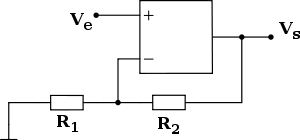
\includegraphics[width=7cm]{ampli_op}
\end{figure}

On a alors dans ce cas $V_+=V_-$ avec $i_-=0$ ce qui mène à 
\begin{eqnarray}
V_e = V_- = R_1 i\hspace{1cm} i = \frac{V_S}{R_1+R_2}\\
&\Longrightarrow& V_e = \frac{R_1}{R_1+R_2}V_S\\
&\Longrightarrow& V_S = \left(1 + \frac{R_2}{R_1}\right)V_e
\end{eqnarray}
on constate donc que si on choisit $R_2\gg R_1$ on va pouvoir nettement amplifier en tension le signal d'entrée $V_e$.\\


On peut faire le diagramme de Bode d'un tel amplificateur, on s'attend à un passe bas du premier ordre. On vérifie ainsi la validité de notre modélisation (considérer l'AOP comme un circuit du premier ordre).\\

On peut ensuite faire varier le rapport $R_2/R_1$ et tracer la fréquence de coupure $f_c$ à -3dB (la repérer en regardant aussi la phase : on a $\phi = 45$° à $f=f_c$) en fonction de $1/A$ où 
\begin{eqnarray}
A = 1 + \frac{R_2}{R_1}
\end{eqnarray}
On s'attend à avoir un produit gain $\times$ bande passante constant ce qui correspond à 
\begin{eqnarray}
f_c \times A = cste \simeq 3\;MHz
\end{eqnarray}
et on s'attend donc à obtenir une droite pour $f_c = f(1/A)$.\\

On voit donc ici que si on veut amplifier sur une grande plage de fréquences on va avoir un faible Gain : on a donc une limitation fréquentielle.

\paragraph{Remarque :} Il existe aussi une limitation en tension aussi : l'amplitude de la tension de sortie est limitée par la tension $V_{sat}$ (légèrement inférieur à $Vcc$.\\

\paragraph{Remarque :}Il existe aussi une limitation en courant aussi : l'AOP ne peut délivrer une intensité de plus de $40$ mA environ.\\

L'AOP bien que simple en apparence et facile à utiliser du point de vue des équations, est en réalité constitué d'une dizaine de transistor. Son comportement est donc compliqué. La prochaine partie concerne l'étude d'un amplificateur de courant basé sur deux transistors, cela va donc nous permettre de visualiser plus clairement le comportement de tels dispositifs.

\section{Amplification en courant}
On suit globalement le TP 2 donné dans le dossier.
\begin{figure}[h]
	\centering 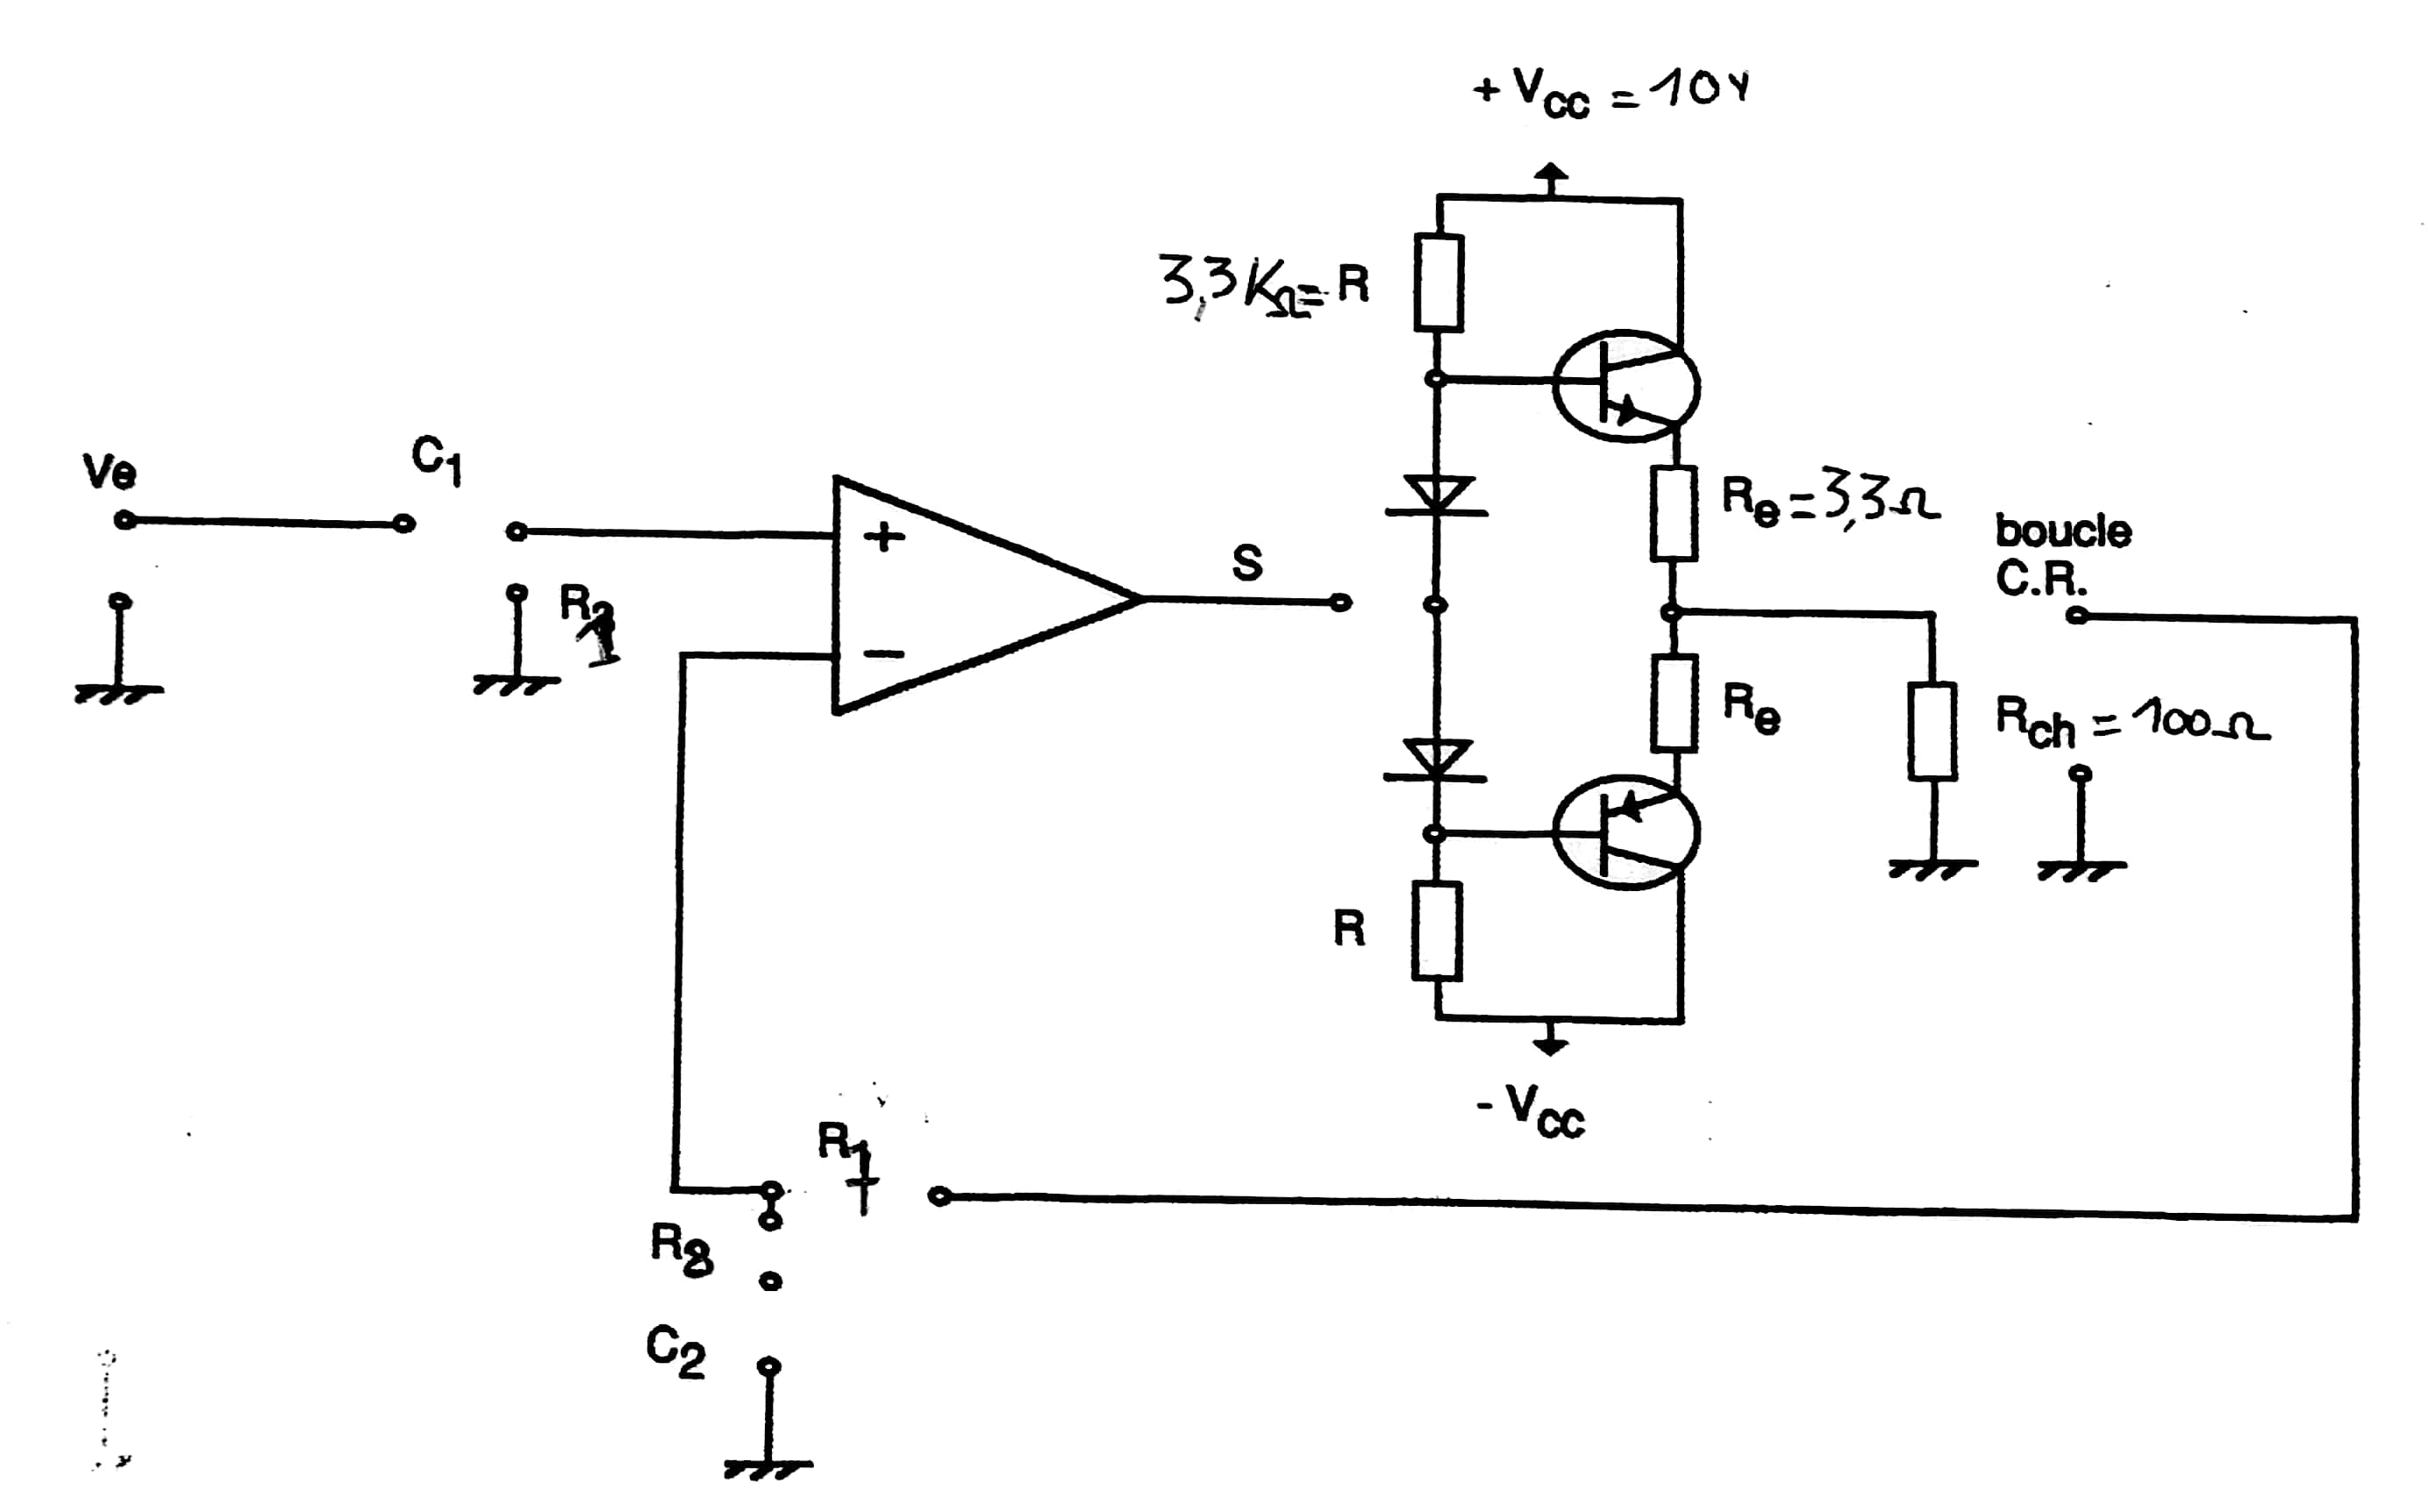
\includegraphics[width=15cm]{ampli}
\end{figure}

\subsection{Amplificateur de classe B}
\paragraph{Applications des ampli courants :} LED (pour régler la luminosité d'une télé, pour régler la portée d'une télécommande infrarouge).\\

On considère le circuit ci dessous, et on enlève les résistances notées $R$ et passe outre les diodes pour ne regarder que l'ampli de classe A. On ne considère pas non plus l'AOP qui sera pour la dernière partie. \\

On a la le cas élémentaire d'un amplificateur de courant de classe B, qui amplifie en courant d'un facteur $\beta \simeq 100$ ($i_e = \beta i_B$).\\
 
Si on regarde à l'oscillo les tensions d'entrée et de sortie $V_e$ et $V_S$ on constate que lorsque $|V_e|$ n'excède pas un certain seuil $V_e^{seuil}$ égal ici à 0,52\,V, la tension de sortie est nulle (c'est dû aux jonctions PN des transistors qu'il faut polariser pour faire passer un courant). On a donc plus une sinusoïde parfaite en sortie, et ainsi si on mesure le taux de distorsion (voir partie 4) on trouve quelque chose de conséquent de l'ordre de quelques \%, ici on mesure $4,6$ \%.\\

On peut de plus mesurer la chute de tension entre entrée et sortie
\begin{eqnarray}
Vpp_s-Vpp_e = 1,37 V
\end{eqnarray}
que l'on peut comparer à $2V_S = 1,05$ V, on voit que ce n'est pas exactement égal, c'est parce que l'on a une chute de tension supplémentaire due aux résistances $R_e$, on a en effet
\begin{eqnarray}
V_e = V_e^{seuil} + R_e i_C + V_S 
\end{eqnarray}
où $i_C$ est le courant en sortie du transistor.\\

 On ne peut pas utiliser cet amplificateur pour amplifier un signal audio par exemple, car bien que le signal soit bel et bien amplifié il est bruité dans un même temps (on voit apparaître de nouvelles harmoniques) à cause de cette tension seuil (tension de polarisation des transistors).
 
 \subsection{Amplificateur de classe AB}
Pour remédier au problème précédent on ajoute deux diodes et les résistances qui vont avec pour que la tension d'entrée soit retransmise quelque soit sa valeur. En effet les diodes sont choisies pour que leur caractéristique soit telle que la tension à leurs bornes soit égale à 0,6 V pour tout courant suffisamment conséquent.\\ On peut alors à nouveau mesurer le taux de distorsion, et on trouve cette fois une valeur inférieure au pourcent : c'est mieux ! (dans la pratique on mesure 0,61\%).\\
\textbf{Remarque :} C'est tout de même plus que le signal délivré par le GBF qui a un taux de distorsion inférieur au dixième de pourcent : ce n'est donc pas parfait non plus.\\

On peut maintenant tracer le rendement
\begin{eqnarray}
\eta = \frac{P_{ch}}{P_+ + P_-} = \frac{V_{ch}^2/R_{ch}}{V_{cc}(\langle I_+ \rangle + \langle I_- \rangle)}
\end{eqnarray}
en fonction de la tension d'entrée $V_e$, où $V_{cc}$ est la tension (continue) d'alimentation des transistors. On mesure les intensité moyennes avec un ampèremètre en DC et la tension efficace avec un voltmètre en AC.\\ 
On s'attend à avoir un rendement croissant avec $V_e$ et ayant une allure parabolique. La courbe s'interrompt lorsque $V_e$ est égale à la tension de saturation : on mesure $V_e^{sat} = 6,7$ V. On atteint donc par la même occasion le rendement maximal : on mesure ici $\eta_{max} = 36,6$ \%. Ce rendement maximal est faible comparé aux $708,5$ \% environ annoncé par le constructeur pour ce push pull, c'est dû au fait que contrairement à ce que l'on pourrait attendre, la tension de sortie sature bien avant atteindre l'amplitude max en théorie qui vaut $Vcc$ = 10 V. En effet lorsque la tension en entrée devient trop grande on a chute une de tension au niveau des diodes, ce qui correspond, lorsque celle la tension aux borne des diodes s'annule complètement, à un courant nul les traversant (on le voit en regardant la caractéristique). Les diodes se comportent donc comme si elles étaient fermées : le circuit est ouvert au niveau des diodes.\\ 
On peut calculer l'expression du $V_S^{max}$ max réel :
\begin{eqnarray}
V_S^{max} + V_{be} + Ri_b = Vcc\\
V_S^{max} = Rch\, i_b = Rch\,\beta i_c\\
\Longrightarrow V_S^{max} = \frac{Rch (Vcc-Vbe)}{Rch + R/\beta} \stackrel{ici}{\simeq} 6,5\,V
\end{eqnarray}

C'est une fois la tension optimale repérée (c'est $V_e^{sat}$ : celle pour laquelle le rendement est maximal) que l'on peut faire une nouvelle mesure du taux de distorsion : on trouve 0,61 \% ce qui est bien mieux que sans les diodes.\\

On peut, comme dans la première partie mesurer le gain et la fréquence de coupure l'amplificateur pouvant être assimilé à un passe bas d'ordre 1. On mesure $G = 0,987$, $f_c = 14$ MHz et donc un produit gain bande $13,8$ MHz : très conséquent.\\

On a donc ici un amplificateur correct puisqu'il amplifie en courant tout en introduisant un taux de distorsion acceptable, le rendement est cependant assez décevant et on sait que c'est dû au diode. On va donc maintenant explorer une autre solution pour s'affranchir des deux problèmes à la fois.

\section{Amplification en puissance}
\paragraph{Applications :} Audio, moteurs...\\

On ajoute un AOP monté en amplificateur de tension non inverseur (tel que présenté dans la première partie) à notre amplificateur de courant, et on retire les diodes, l'AOP . On amplifie donc en courant \textbf{et} en tension : on réalise de l'amplification de puissance à proprement parler, tout en s'affranchissant du problème de rendement précédent.

\begin{figure}[h]
	\centering 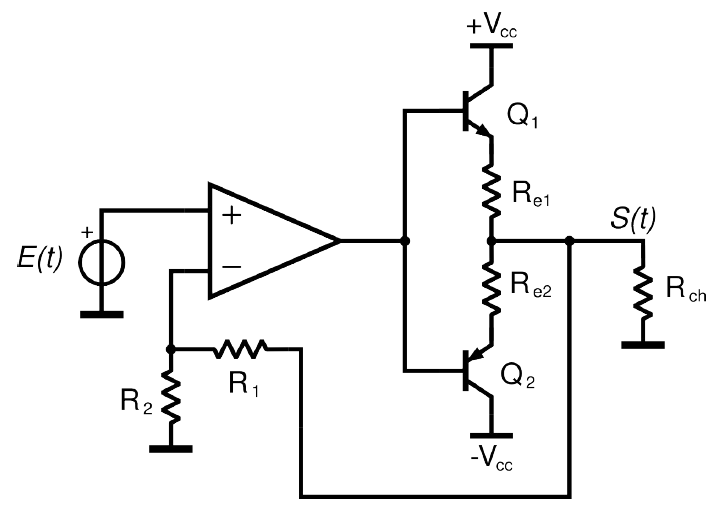
\includegraphics[width=10cm]{p3}
\end{figure}

On peut à nouveau tracer 
\begin{eqnarray}
\eta = f(V_e) 
\end{eqnarray}
et identifier le rendement max. On va ici simplement identifier la tension de saturation et le rendement max : on mesure $\langle I_+ \rangle = 26,14$ mA, $\langle I_- \rangle = 24,93$ mA, $V_S^{eff} = 5,26$ V avec la tension de saturation $V_e^{sat}$ = 2,02V. Cela correspond au rendement 
\begin{eqnarray}
\eta =  \frac{V_{ch}^2/R_{ch}}{V_{cc}(\langle I_+ \rangle + \langle I_- \rangle)} = 54,7 \%
\end{eqnarray}
ce qui est bien mieux que avec les diodes et sans AOP.\\

Pour pousser la comparaison il faut tout de même regarder le taux de distorsion : on mesure 0,18\% ce qui est encore mieux qu'avec les diodes. On a donc à la fois un meilleur rendement et un bon taux de distorsion : notre amplificateur commence à se montrer performant !\\

\textbf{Remarque :} Si on conserve les diodes, on a pas d'amélioration du rendement, mais on obtient un taux de distorsion de $0,01$\% ce qui est excellent.\\ 

On peut là encore mesurer le gain et la fréquence de coupure l'amplificateur + AOP pouvant tout deux être assimilés à des passe bas d'ordre 1. On mesure $G = 7,06$, $f_c = 380$ kHz et donc un produit gain bande $2,68$ kHz : beaucoup plus faible que pour l'ampli en courant seul.\\
$\longrightarrow$ on amplifie donc plus en puissance mais on perd en plage de fréquence utilisable.


\subsection*{Impédances d'entrée et de sortie}
Si on veut savoir à quel types d'appareil on peut brancher notre amplificateur il faut connaître son impédance d'entrée de sortie. Pour cela on travaille comme sur le schéma suivant,
\begin{figure}[h]
	\centering 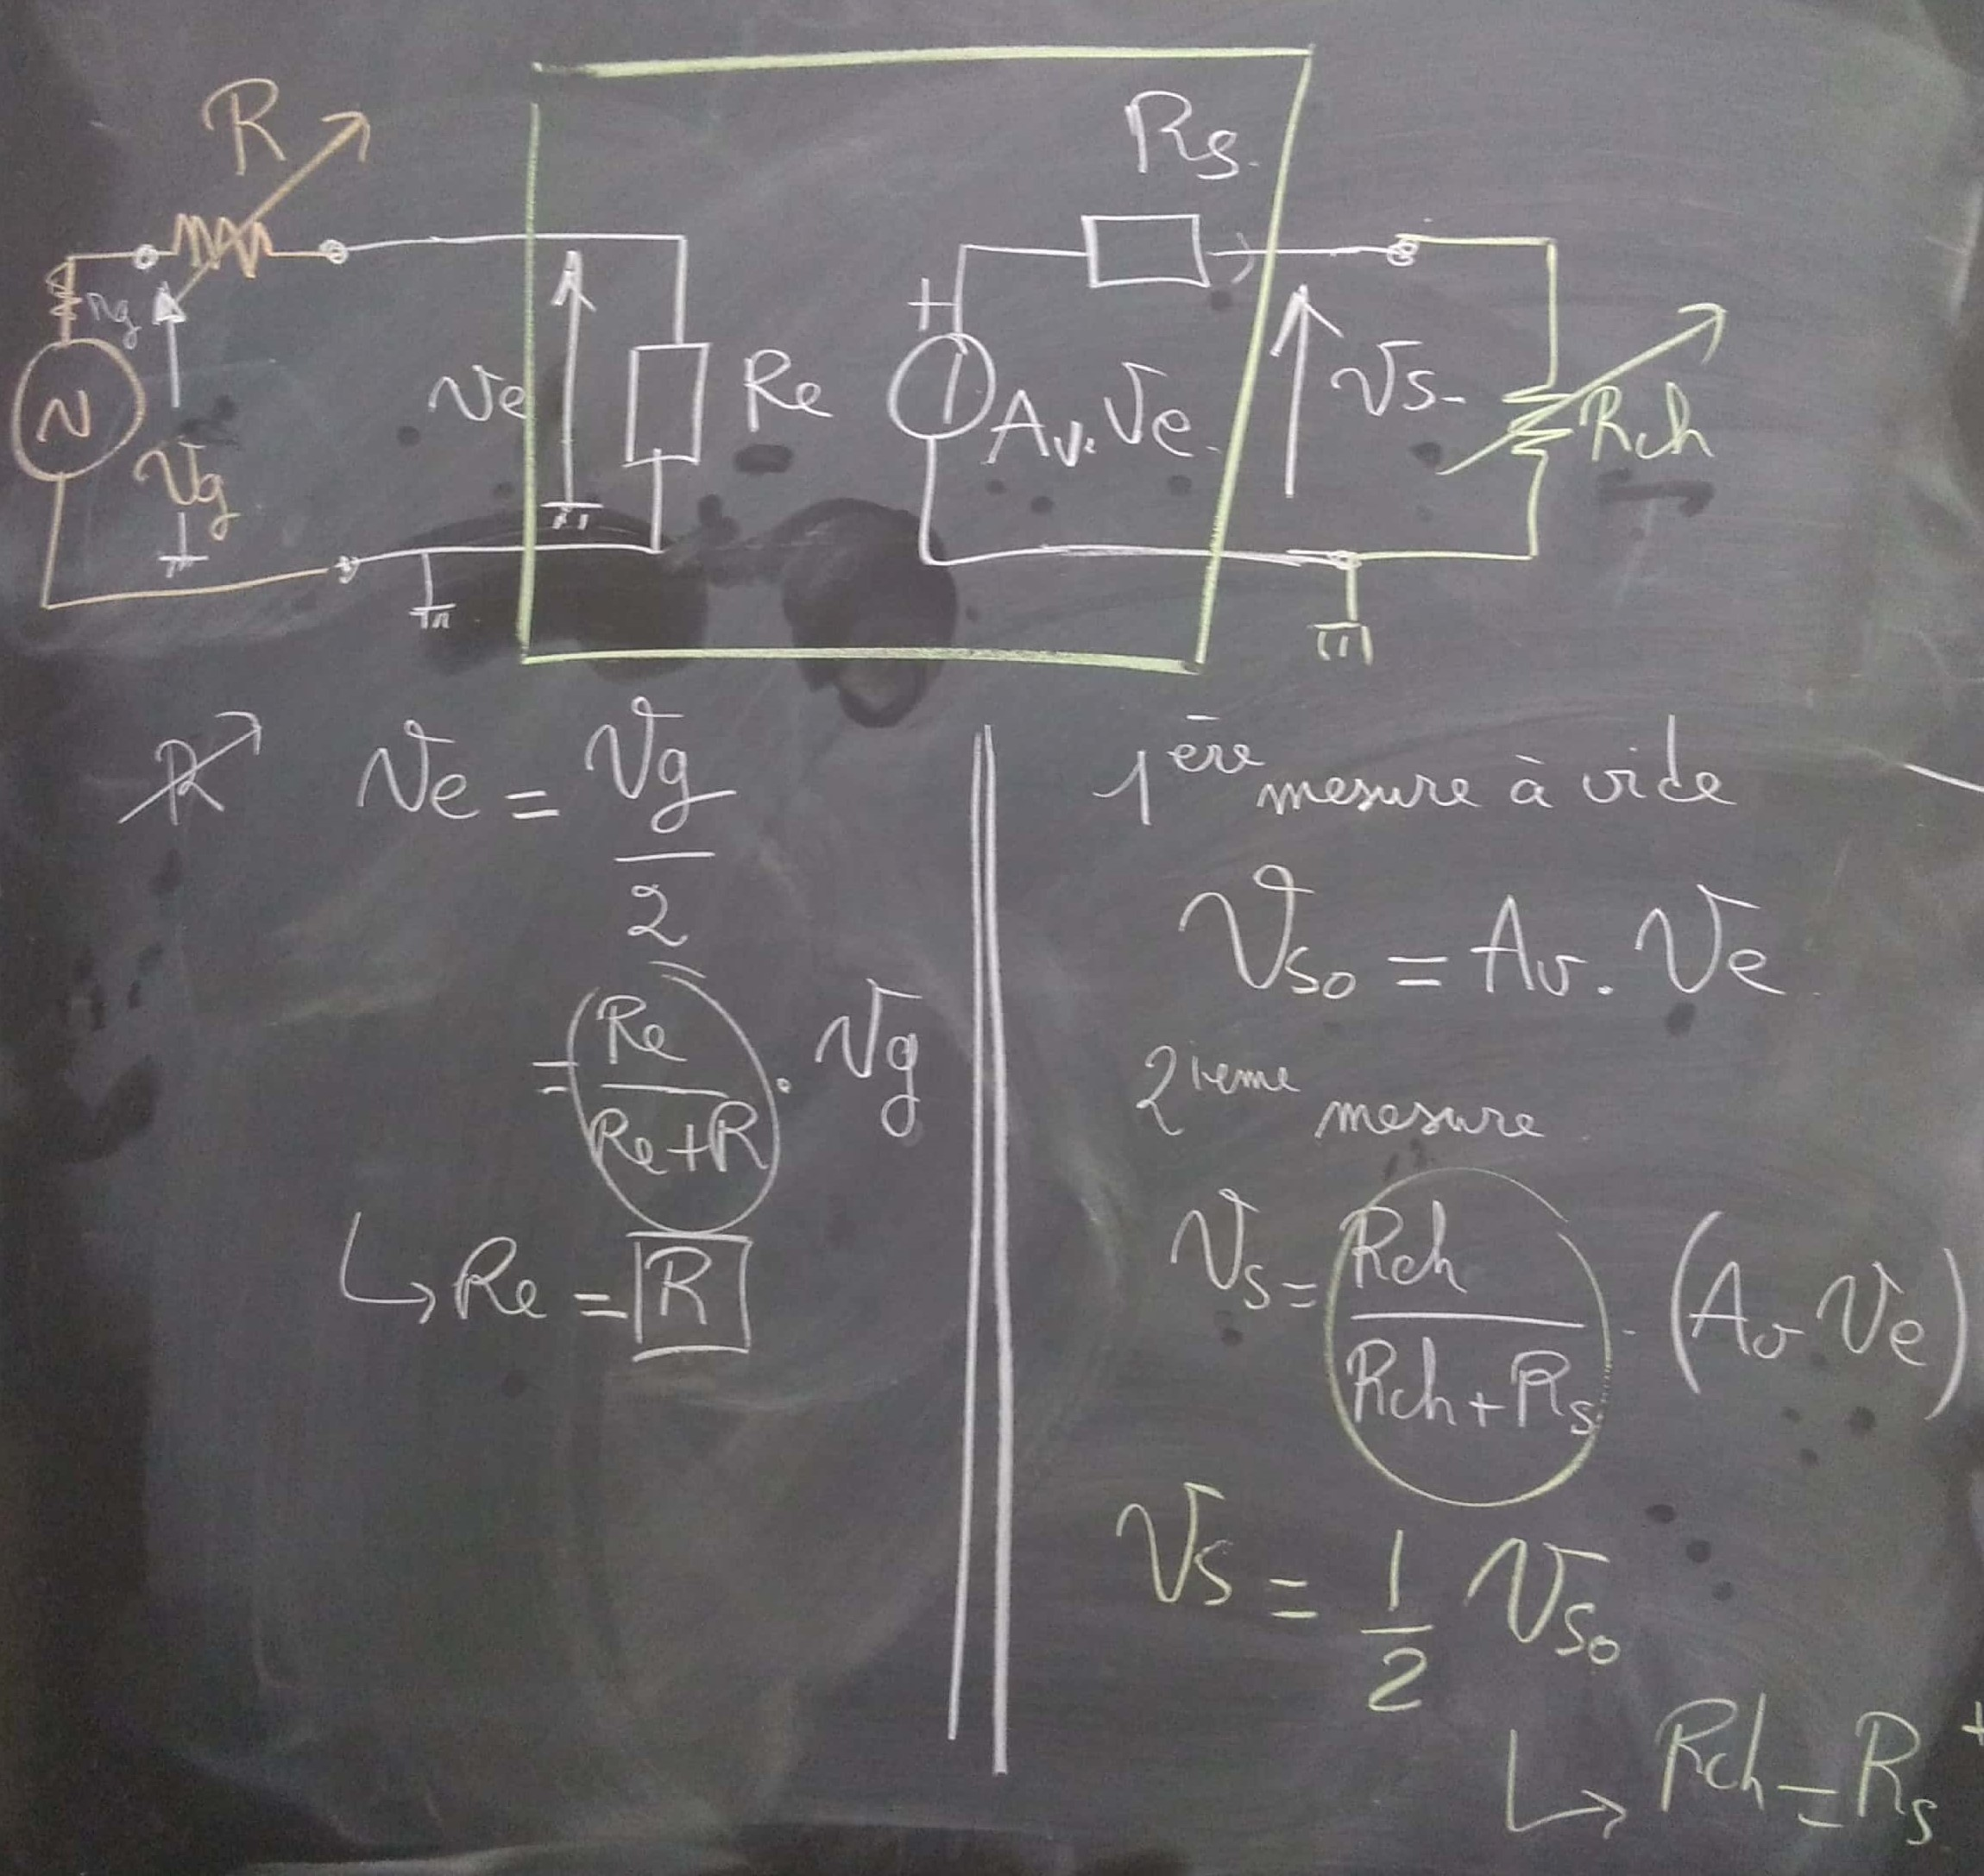
\includegraphics[width=10cm]{impedance}
\end{figure}
où le schéma type en haut représente l'amplificateur, avec l'entrée à gauche et la sortie à droite. Ici on mesure $R_e= 850$ k$\Omega$ et $R_S = 0,6\,\Omega$. Cela n'a rien de surprenant car on s'attend à ce que ces impédances correspondent à celles de l'AOP qui "entoure" notre circuit.

\section{Notice pour le distorsiomètre}
\begin{figure}[h]
	\centering 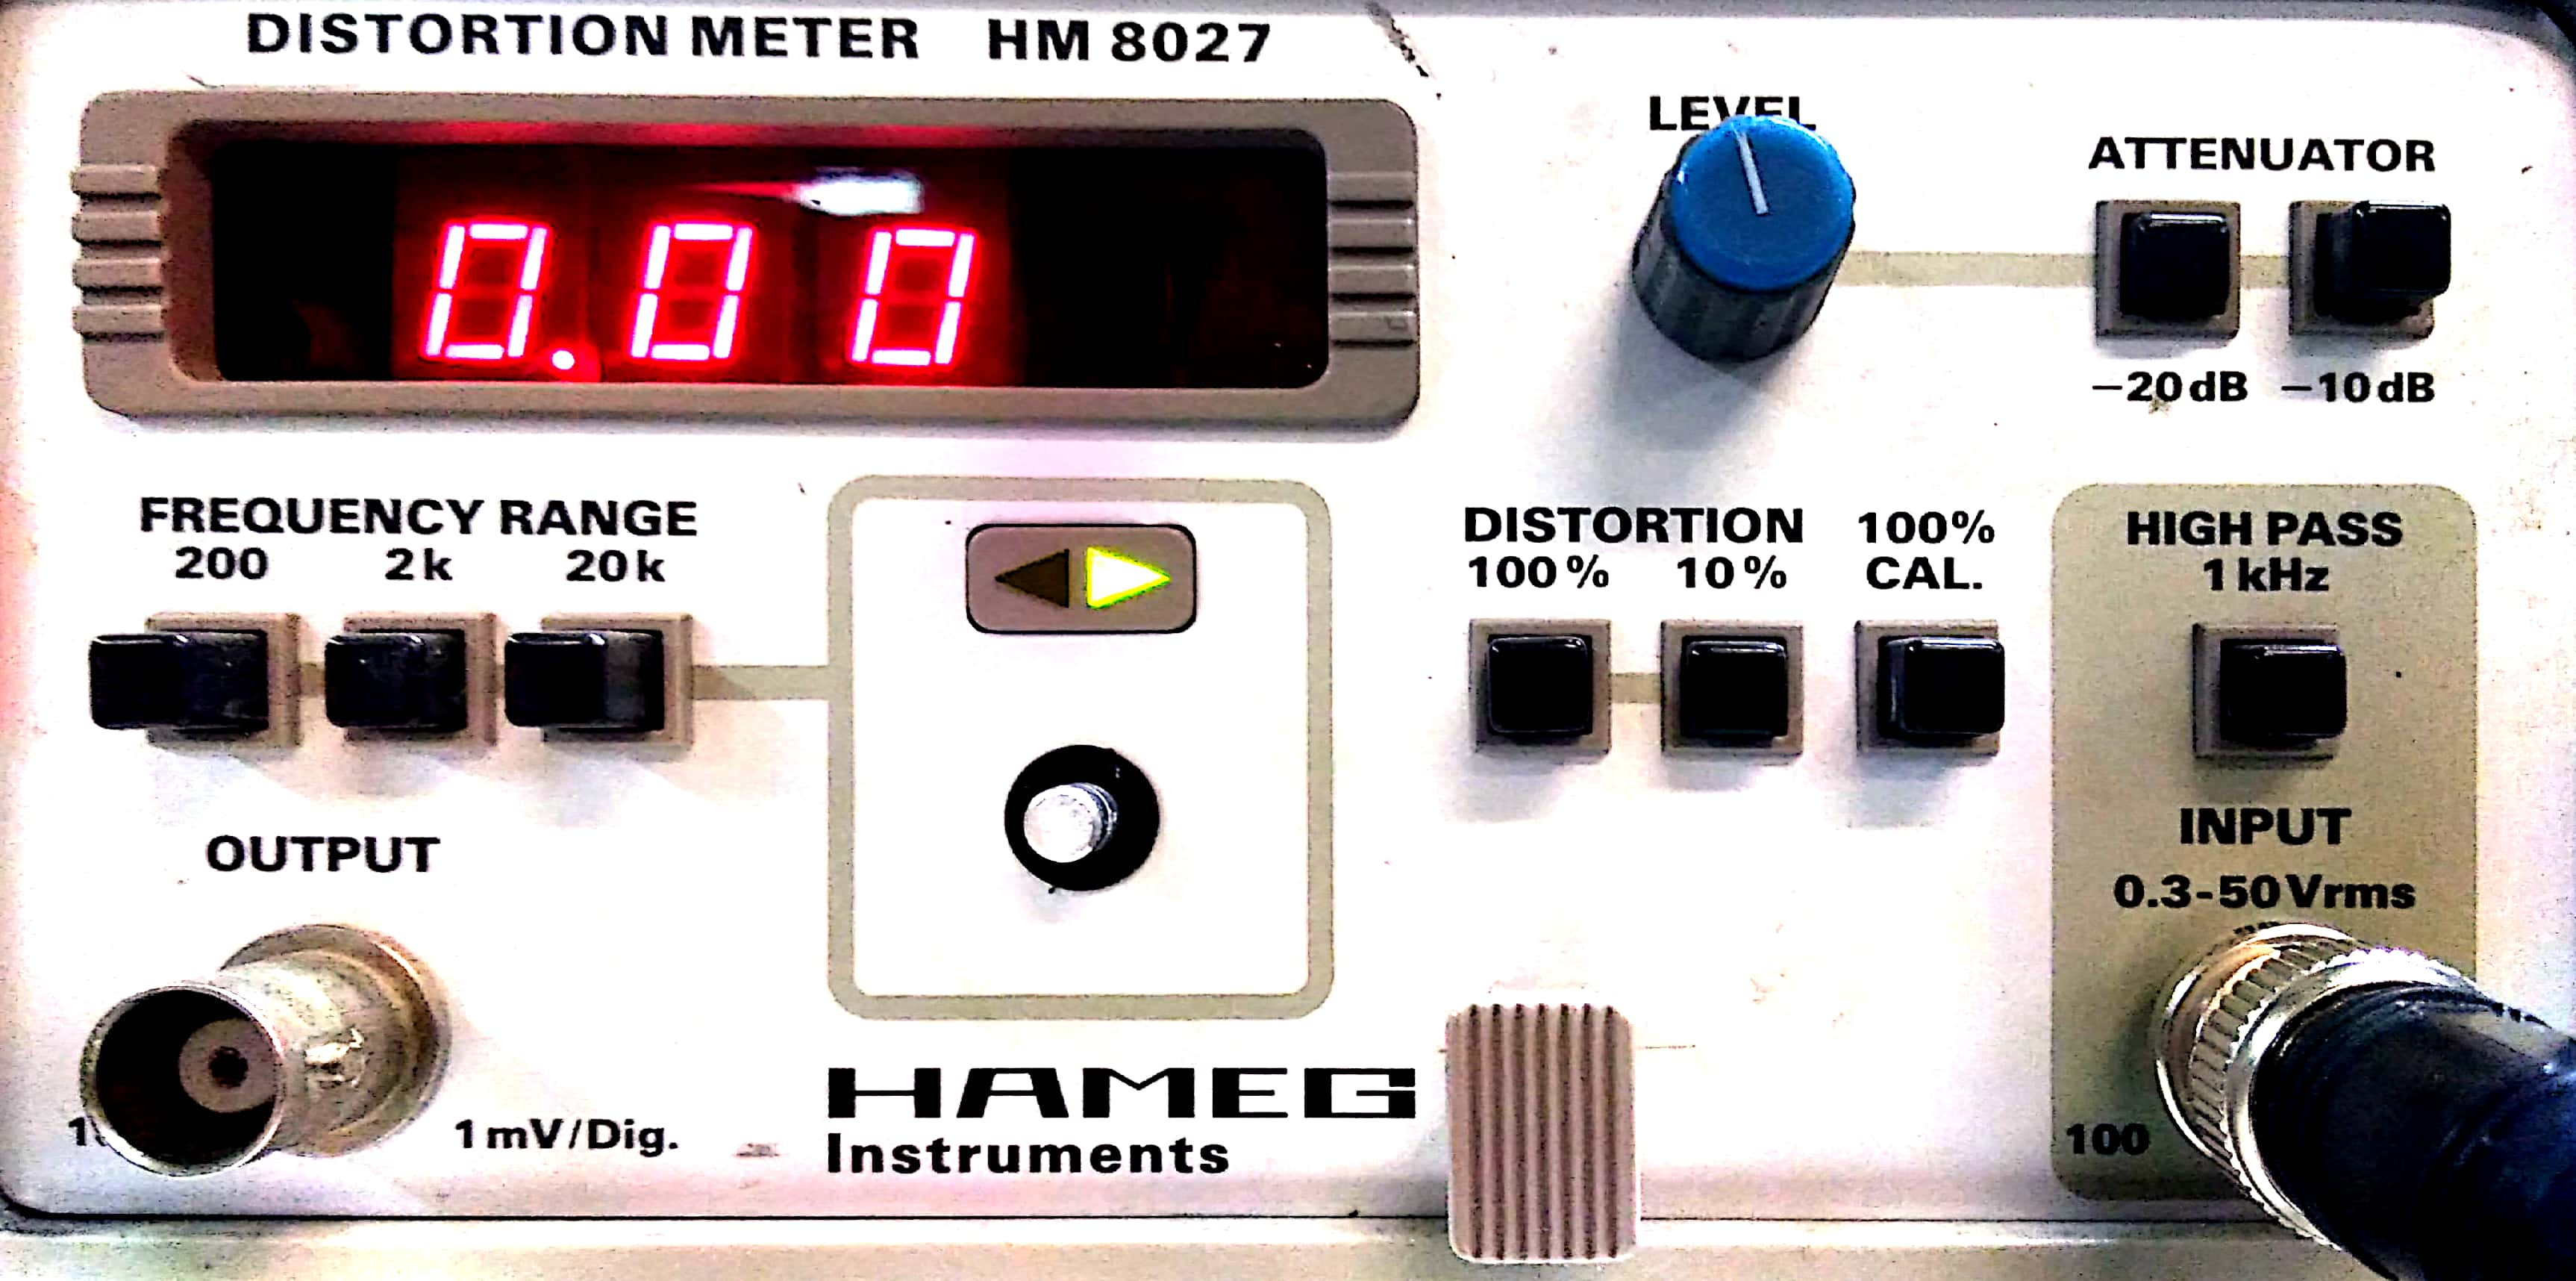
\includegraphics[width=13cm]{distorsiometre}
\end{figure}
On branche le signal à analyser sur l'entrée input. On appuie sur \textbf{100\% cal} et on règle le calibrage à 100 avec le bouton \textbf{level}. On appuie ensuite sur le bouton \textbf{frequency range} correspondant à la plage dans laquelle se trouve notre fondamentale (200 pour la plage de 0 à 200Hz, 2k pour la plage de 200 à 2000Hz et 20k de 2k à 20k). On tourne ensuite le petit bouton métallique sous les deux flèches vertes, jusqu'à éteindre les deux flèches. On appuie finalement sur \textbf{distorsion 100\%} pour afficher le taux de distorsion. On accède à un digit de plus en appuyant sur \textbf{10\%} (distorsion). 

 
\end{document}